\documentclass[twoside]{article}
\setlength{\oddsidemargin}{0.25 in}
\setlength{\evensidemargin}{-0.25 in}
\setlength{\topmargin}{-0.6 in}
\setlength{\textwidth}{6.5 in}
\setlength{\textheight}{8.5 in}
\setlength{\headsep}{0.75 in}
\setlength{\parindent}{0 in}
\setlength{\parskip}{0.1 in}

\usepackage{graphicx}
\usepackage{url}

%
% The following commands sets up the lecnum (lecture number)
% counter and make various numbering schemes work relative
% to the lecture number.
%
\newcounter{lecnum}
\renewcommand{\thepage}{\thelecnum-\arabic{page}}
\renewcommand{\thesection}{\thelecnum.\arabic{section}}
\renewcommand{\theequation}{\thelecnum.\arabic{equation}}
\renewcommand{\thefigure}{\thelecnum.\arabic{figure}}
\renewcommand{\thetable}{\thelecnum.\arabic{table}}
\newcommand{\dnl}{\mbox{}\par}

%
% The following macro is used to generate the header.
%
\newcommand{\lecture}[4]{
  \pagestyle{myheadings}
  \thispagestyle{plain}
  \newpage
  \setcounter{lecnum}{#1}
  \setcounter{page}{1}
  \noindent
  \begin{center}
  \framebox{
     \vbox{\vspace{2mm}
   \hbox to 6.28in { {\bf COMPSCI~630~~~Systems
                       \hfill Spring 2017} }
      \vspace{4mm}
      \hbox to 6.28in { {\Large \hfill Lecture #1: #2  \hfill} }
      \vspace{2mm}
      \hbox to 6.28in { {\it Lecturer: #3 \hfill Scribe(s): #4} }
     \vspace{2mm}}
  }
  \end{center}
  \markboth{Lecture {#1}: #2}{Lecture {#1}: #2}
  \vspace*{4mm}
}

%
% Convention for citations is authors' initials followed by the year.
% For example, to cite a paper by Leighton and Maggs you would type
% \cite{LM89}, and to cite a paper by Strassen you would type \cite{S69}.
% (To avoid bibliography problems, for now we redefine the \cite command.)
%
\renewcommand{\cite}[1]{[#1]}

% \input{epsf}

%Use this command for a figure; it puts a figure in wherever you want it.
%usage: \fig{NUMBER}{FIGURE-SIZE}{CAPTION}{FILENAME}
\newcommand{\fig}[4]{
           \vspace{0.2 in}
           \setlength{\epsfxsize}{#2}
           \centerline{\epsfbox{#4}}
           \begin{center}
           Figure \thelecnum.#1:~#3
           \end{center}
   }

% Use these for theorems, lemmas, proofs, etc.
\newtheorem{theorem}{Theorem}[lecnum]
\newtheorem{lemma}[theorem]{Lemma}
\newtheorem{proposition}[theorem]{Proposition}
\newtheorem{claim}[theorem]{Claim}
\newtheorem{corollary}[theorem]{Corollary}
\newtheorem{definition}[theorem]{Definition}
\newenvironment{proof}{{\bf Proof:}}{\hfill\rule{2mm}{2mm}}

% Some useful equation alignment commands, borrowed from TeX
\makeatletter
\def\eqalign#1{\,\vcenter{\openup\jot\m@th
 \ialign{\strut\hfil$\displaystyle{##}$&$\displaystyle{{}##}$\hfil
     \crcr#1\crcr}}\,}
\def\eqalignno#1{\displ@y \tabskip\@centering
 \halign to\displaywidth{\hfil$\displaystyle{##}$\tabskip\z@skip
   &$\displaystyle{{}##}$\hfil\tabskip\@centering
   &\llap{$##$}\tabskip\z@skip\crcr
   #1\crcr}}
\def\leqalignno#1{\displ@y \tabskip\@centering
 \halign to\displaywidth{\hfil$\displaystyle{##}$\tabskip\z@skip
   &$\displaystyle{{}##}$\hfil\tabskip\@centering
   &\kern-\displaywidth\rlap{$##$}\tabskip\displaywidth\crcr
   #1\crcr}}
\makeatother

% **** IF YOU WANT TO DEFINE ADDITIONAL MACROS FOR YOURSELF, PUT THEM HERE:



% Some general latex examples and examples making use of the
% macros follow.

\begin{document}

%FILL IN THE RIGHT INFO.
%\lecture{**LECTURE-NUMBER**}{**DATE**}{**LECTURER**}{**SCRIBE**}
\lecture{18}{April 28}{Emery Berger}{Manish Motwani, Sam Baxter}

\section{Times, Clocks, and Stuff Like That}

One of the major issues in distributed systems is dealing with time because the
assumption (made in everyday activites) that time is universal doesn't hold
true. This is because latency in communication can cause non-deterministic
ordering of events and clocks to fall out of sync.

If we could attach a \emph{perfect} timestamp to each event occurence, we could
obtain a \emph{total order} on those events. Unfortunately, perfect timestamps
are infeasible in distributed systems because the latency of message passing
communication and clock drift forces the loss of synchronization.

\subsection{How are clocks synchronized?}
\begin{enumerate}
    \item Atomic Clocks - The most accurate time measuring device. Uses the
        frequency of transmission of atoms under some light in the
        electromagnetic spectrum as a frequency standard for timekeeping. These
        are expensive (costs \$25000) and are not practical for large
        or personal deployments.
    \item Quartz Crystal - Quartz is known to vibrate at a certain frequency
        under some electronic oscillator. This creates a precise signal that
        produces a much more accurate clock than digital clocks, but less
        accurate than atomic clocks. The synchronization problem still persists,
        and several quartz clocks can drift further and further apart.
\end{enumerate}
The time delay in synchronizing these clocks is nondeterministic. The
\emph{Network Time Protocol} (NTP) is a common standard for synchronizing the
clocks of moder distributed servers. However, this synchronization is
coarse-grained (i.e. clocks may be guaranteed to be within a day, hours,
minutes, or seconds of sync with one another, but not fine-grained enough to
guarantee against inversions in the perceived order of events).

Lamport described a way to determine a global ordering of events in a
distributed system by defining a "happens-before" relationship between two
events, establishing a \emph{total order}. Lamport used \emph{logical clocks}
(a.k.a. Lamport clocks), which are essentially global counters (as opposed to
perfect timestamps) that increment each event and are transmitted to all parts
of a distributed system in every communication.

\subsection{Vector Clocks}
Vector clocks generalize Lamport clocks by maintaining essentially a vector of
logical clocks, one for each thread or process in the distributed system. A
vector clock must be maintained for \emph{each} variable in the program. They
encode the happens-before relation on all variable accesses/modifications,
establishing a total order on these events.

Consider the following example.

\begin{center}
    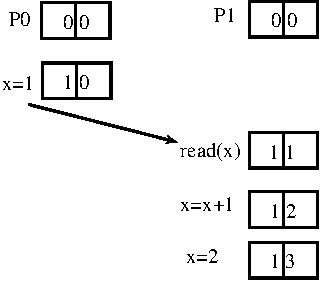
\includegraphics[scale=.75]{example1.pdf}
\end{center}

In this example, two processes ($P_0$ and $P_1$) operate on a shared variable $x$.
Each process maintains a vector clock of size 2 (since there are two processes)
intialized to $[0|0]$. After operation $x=1$ in $P_0$, its vector clock is
updated to $[1|0]$ and at this point $P_1$ takes over execution. $P_0$ passes
its vector clock $[1|0]$ to $P_1$. Before $P_1$ executes any instructions, it
compares its vector clock $[0|0]$ against $P_0$'s vector clock $[1|0]$. As the
entry in $P_1$'s vector clock for $P_0$ is less than or equal to the entry of
$P_0$ in its vector clock (i.e. $0\le1$), there is no race condition. In
general, if there does not exist a happens-before relation between two events
there could be a potential race. Logical and vector clocks detect such race
conditions.

\subsection{Race Detection}
The happens-before relation can be used to detect potential race conditions in
variable accesses and modifications. Vector clocks encode this relationship, so
they lend to a \emph{precise} notion of race-detection (i.e. if a race were to
occur, it would be detected, and any races it detects are legitimate, potential
races).

With the precision of vector clocks comes performance overhead. They require
$O(n)$ space (linear in the number of threads/processes) per variable and vector
clock operations (comparisons to determine ordering) are $O(n)$ time as as they
require a linear traversal of the vectors.

\subsection{Alternative Approaches to Race Detection}
To address the performance overhead of vector clocks, some techniques sacrifice
precision. ERASER is a Java race detector that uses such an approach, employing
a \emph{LockSet} analysis algorithm to detect potential races (potentially
giving false-positives). The key insight here is that if multiple processes work
on a shared variable without holding a lock, then there is a potential race. As
an example, consider the two processes below:

\begin{center}
    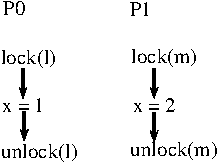
\includegraphics[scale=.75]{example2.pdf}
\end{center}

Initially, we consider the LockSets for each process to be empty (i.e. $LS(P_0)
= LS(P_1) = \emptyset$). After $P_0$ and $P_1$ acquire the locks $l$ and $m$
respectively, the lock-sets for the variable assignment on each process will be
$LS(P_0) = \{l\}$ and $LS(P_1) = \{m\}$. Since $LS(P_0)\cap LS(P_1) =
\emptyset$, there is a potential race condition. In general, the LockSet
analysis reports a potential race whenever the intersection is empty.

Why is this a \emph{potential} race?
\begin{enumerate}
    \item The race could be benign, if for instance both threads assign the same
        value to $x$.
    \item Note that if programs use alternative means of establishing ordering
        (rather than locking primitives), LockSet cannot detect that they may
        remain mutually exclusive.
\end{enumerate}


\subsection{FastTrack - Prof. Stephen Freund Guest Lecturer}
FastTrack gives the precision of vector clocks without the space/time overhead
required by that technique. Freund exploited the realization that in the
majority of scenarios, we only need to remember the \emph{very last write} to a
shared variable instead of a vector clock encoding its entire history. As long
as a race has yet to be detected, there is still a total order on writes, and so
FastTrack replaces linear-sized vector clocks with an \emph{epoch} encoding the
thread id and counter of the last write to a variable. This preserves the
happens-before relation before any races have occured, so FastTrack guarantees
that it will precisely detect at least the first race to occur on a variable.

\subsection{Improving Upon FastTrack}
How can we perform better? We could:
\begin{enumerate}
    \item Sample windows for potential races instead of every variable access.
        This has the downside of not being precise.
    \item Use LockSet analysis until you would report a potential race, then
        switch to FastTrack to verify it is not a false positive. Results were
        not as promising as one might hope.
    \item Reduce redundancy in consistency checks. This approach is taken in
        \emph{RedCard}. If a variable is accessed multiple times inside a locked
        critical section that respects the happens-before relation, we can
        perform just a single check instead of checking at each access. Static
        analysis can be used to improve a dynamic detector by recognizing these
        cases.
    \item Looping over an entire array checks accesses to every element in the
        array. If all your program ever does is loop over the entire array, a
        single check can be performed on the array itself, instead of requiring
        checks on every element within it. This involves recognizing access
        patterns and optimizing shadow representations of the happens-before
        relation.
    \item Don't perform the check exactly when the access occurs. This can do
        things like hoist a check out of a loop so it's only done once instead
        of linearly in the number of the iterations.
\end{enumerate}



\end{document}
